\par Les membres du groupe responsables de cette partie étaient Antoine Vallée et Antoine Pietri.

\par Depuis la seconde soutenance, nous faisons progresser un site web en lui ajoutant au fur et à mesure du contenu.
Nous avons depuis le début une page de news que nous mettons régulièrement à jour :

\begin{center}
	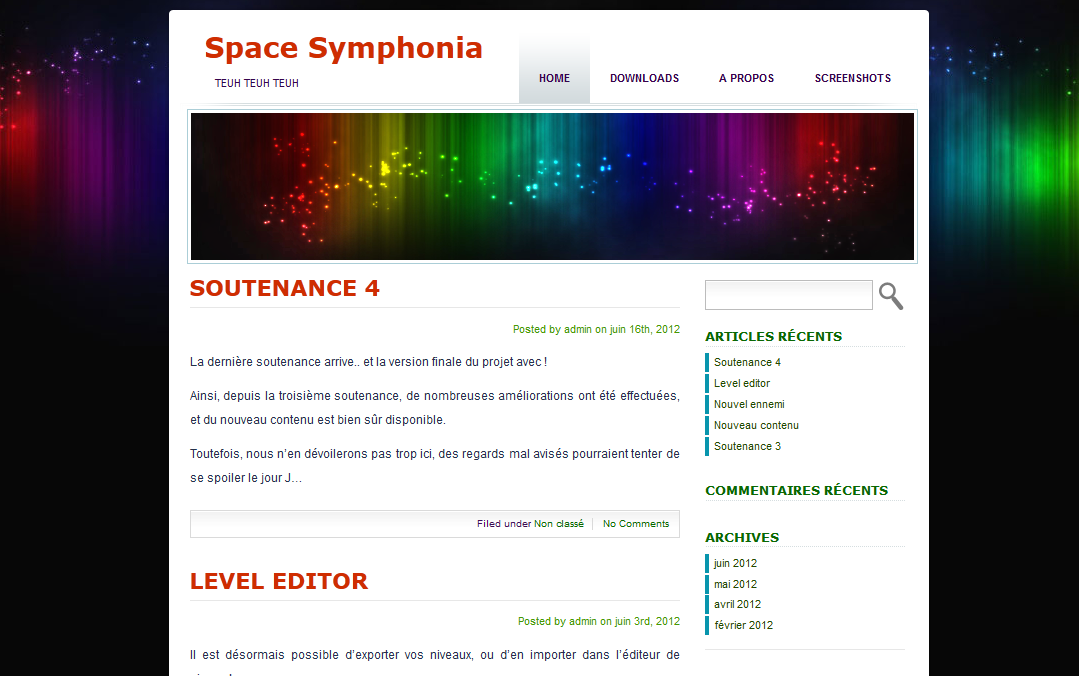
\includegraphics[width=9cm]{images/site1.png}
\end{center}

\par Nous avons peu à peu rajouté une section « Téléchargements » où il est possible de récupérer les sources, l'exécutable et l'installateur : 

\begin{center}
	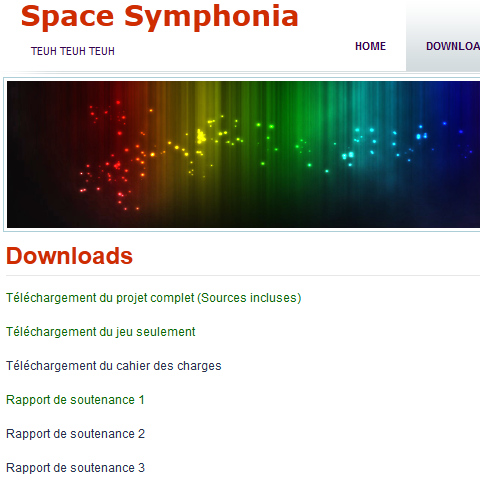
\includegraphics[width=9cm]{images/site2.png}
\end{center}

Puis également une section « À propos » où vous pouvez trouver des informations de contact:

\begin{center}
	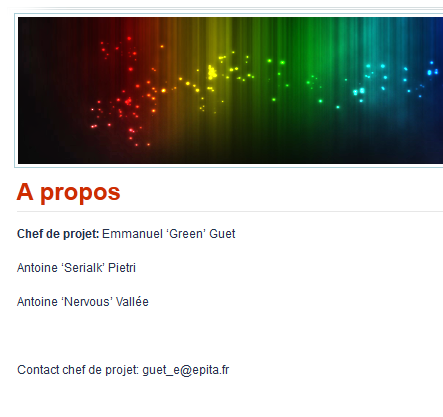
\includegraphics[width=9cm]{images/site3.png}
\end{center}

Et enfin une section « Screenshots » où l'on peut voir différentes captures d'écran qui montrent l'évolution de notre jeu :

\begin{center}
	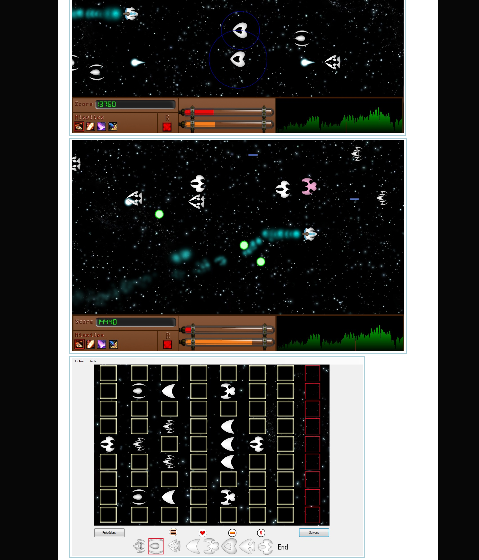
\includegraphics[width=9cm]{images/site4.png}
\end{center}

Le site est une installation Wordpress de base hébergée sur un VPS (Virtual Private Server) tournant sur une Debian Squeeze (avec php5 et lighttpd) administrée par Antoine Pietri. Nous avons acheté le domaine space-symphonia.fr et redirigé vers ce VPS, qui, via lighttpd, le route vers notre site.